%\documentclass[11pt]{article}
\documentclass{ctexart}
\usepackage{amsmath, amssymb}
\usepackage{geometry}
\usepackage{graphicx}

% Set page margins
\geometry{margin=1in}

\title{Partial Differential Equations 偏微分方程}
\author{Yang transcribed by Handwriting of Prof Langemann}
\date{07.11.2023}

\begin{document}

\maketitle


\section*{I.1. 扩散和热传导}
考虑域 \( \Omega \subseteq \mathbb{R}^d \) 内的位置 \( \vec{x} \)(\( \Omega \) 是开集!),
其中 \( d=1 \) 对应于通道或导线,\( d=2 \) 对应于板,\( d=3 \) 对应于实际空间。
对于时间 \( t \geq 0 \),令 \( u = u(t, \vec{x}) \) 表示浓度或温度,这是两个独立的物理量。
令 \( \vec{I} = \vec{I}(t,\vec{x}) \in \mathbb{R} \) 表示材料或热通量。

\textbf{本构方程 / 材料方程:}
\begin{enumerate}
\item 均匀材料(与 \( \vec{x} \) 无关)各向同性(与方向无关),通量 \( \vec{I} \) 由 \( \vec{I} = -a \nabla u \) 给出,其中 \( a > 0 \) 代表热传导或扩散系数。
\item 非均匀各向同性材料,\( \vec{I} = -a(\vec{x}) \nabla u \),其中 \( a(\vec{x}) \geq \epsilon > 0 \) 对于某个 \( \epsilon \)。
\item 非均匀各向异性材料。
\end{enumerate}

\subsection*{非均匀各向异性材料}

对于非均匀各向异性材料,热或材料通量 \( \vec{I} \) 给定为:
\[ \vec{I} = -A(\vec{x}) \nabla u \]
矩阵 \( A(\vec{x}) \in \mathbb{R}^{d \times d} \) 满足:
\[ \vec{v}^T A(\vec{x}) \vec{v} > 0 \quad \text{对于所有} \quad \vec{v} \neq \vec{0} \]
这意味着 \( A(\vec{x}) \) 是正定的。

此外,我们假设:
\[ \vec{I} \cdot \nabla u < 0 \quad \text{对于所有} \quad \nabla u \neq \vec{0} \]
这通常是物理系统的情况,其中通量倾向于减小梯度(例如,热从热区流向冷区)。

我们还考虑 \( A(\vec{x}) \) 的谱,表示为 \( \text{spec} \, A(\vec{x}) \),满足:
\[ \text{spec} \, A(\vec{x}) \geq \varepsilon > 0 \]

\textbf{备注:}
对于矩阵 \( A(\vec{x}) \) 对梯度向量 \( \nabla u \) 的作用,考虑了其对称性。对于向量 \( \nabla u = \begin{pmatrix} 1 \\ 0 \end{pmatrix} \),得到的通量 \( \vec{I} \) 与 \( A(\vec{x}) \) 的第一列成比例,具体为 \( \vec{I} = - \begin{pmatrix} a_{11} \\ a_{21} \end{pmatrix} \)。

\subsection*{连续性方程}

考虑子域 \( O \subseteq \Omega \),\( O \) 中的总材料或能量由以下表示:
\[ E = \int_O u \, da \]

对于维度 \( d = 2 \),随时间变化的 \( E \) 为:
\[ \frac{dE}{dt} = \frac{d}{dt} \int_O u \, da = \int_O \frac{\partial u}{\partial t} \, da \]

另一方面,由于越过边界的流动引起的 \( E \) 的变化由以下给出:
\[ \frac{dE}{dt} = -\int_{\partial O} \vec{I} \cdot \vec{n} \, ds = -\int_O \nabla \cdot \vec{I} \, da \]
其中 \( \vec{I} \) 是流动矢量,\( \vec{n} \) 是边界 \( \partial O \) 上的外法向矢量。

因此,连续性方程可以表示为:
\[ \int_O \frac{\partial u}{\partial t} \, da = -\int_O \nabla \cdot \vec{I} \, da \]
对于每个独立于材料的 \( O \),导致:
\[ \frac{\partial u}{\partial t} + \nabla \cdot \vec{I} = 0 \]

\begin{figure}
    \centering
    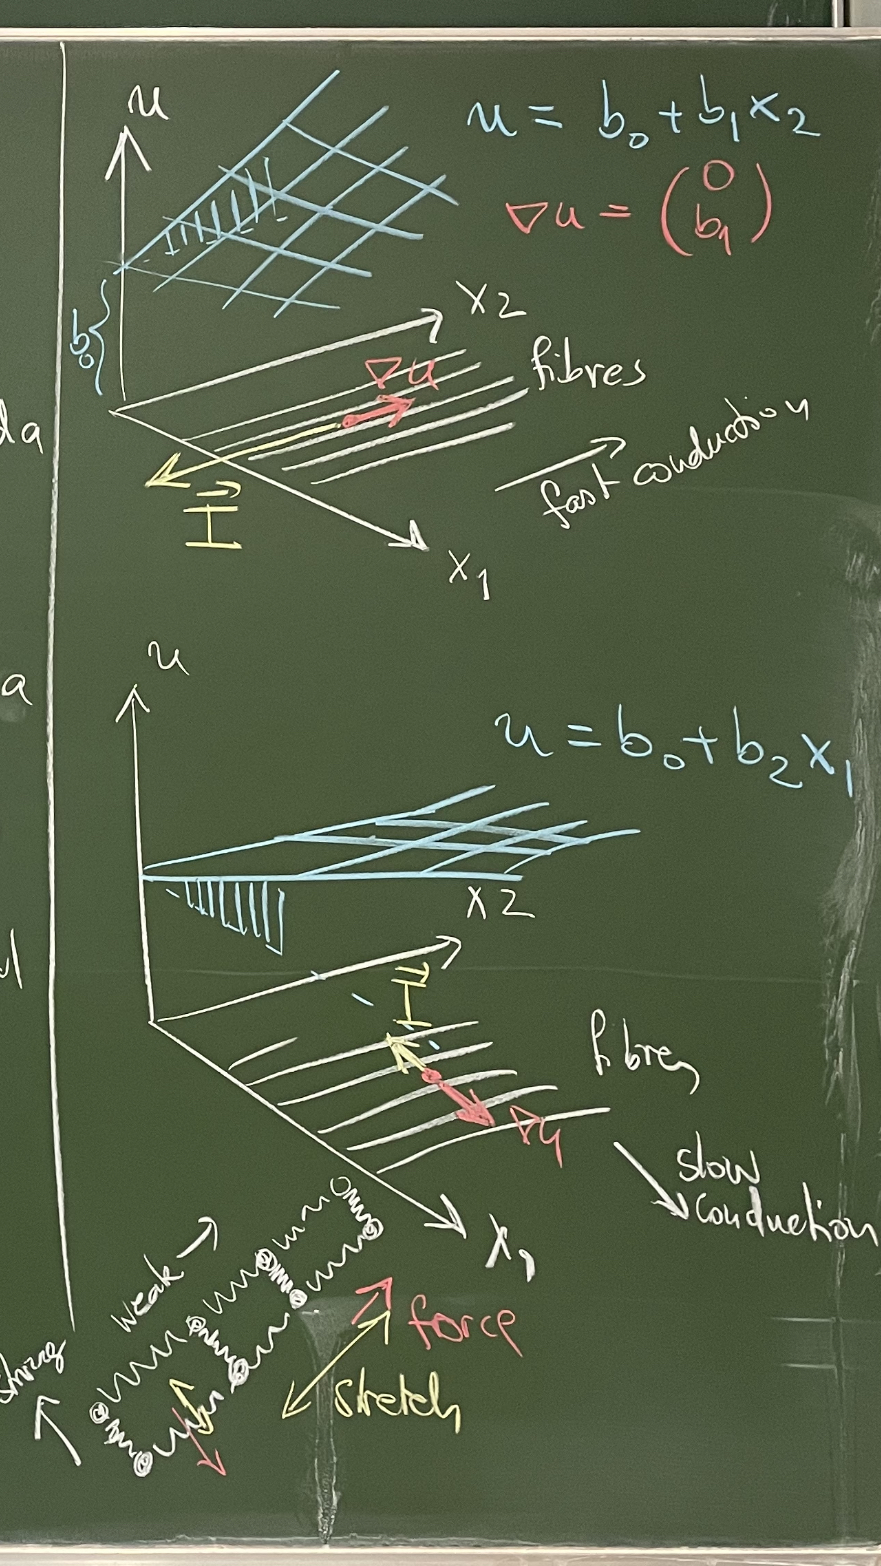
\includegraphics[width=0.5\linewidth]{IMG_2734.jpeg}
    \caption{热传导和力分布}
    \label{fig:enter-label}
\end{figure}

\newpage
\date{15.11.2023.PDE}


\section*{热传导方程的初边值问题}

\subsection*{定义域与边界条件}
考虑定义在域 \( \Omega \) 上的热传导方程,边界 \( \partial \Omega \) 由 \( \Gamma_1 \) 和 \( \Gamma_2 \) 组成,并且 \( \Gamma_1 \cap \Gamma_2 = \varnothing \)。其中,\( \Gamma_1 \) 是固定值边界条件(Dirichlet边界条件),\( \Gamma_2 \) 是给定通量的自然边界条件(Neumann边界条件)。

\subsection*{初边值问题(IBVP)}
热传导方程可以表示为:
\[
u_t = \nabla \cdot [A(x) \nabla u] + f(t,x) \quad \text{对于} \quad x \in \Omega, t > 0
\]
这里 \( u \) 表示温度随时间和空间的变化。

边界条件(BC)分为以下几种:
\begin{itemize}
  \item 在 \( \Gamma_1 \) 上 \( u(t,x) = g(t,x) \) 对于 \( t > 0 \);
  \item 在 \( \Gamma_2 \) 上 \( \boldsymbol{n}^T [A(x) \nabla u] = p(t,x) \) 对于 \( t > 0 \);
  \item 在 \( \Omega \) 上的初始条件 \( u(0,x) = u_0(x) \)。
\end{itemize}

\subsection*{质量守恒(或能量守恒)}
总质量或总能量 \( E \) 是通过 \( \Omega \) 上 \( u \) 的积分给出的:
\[
E = \int_\Omega u \, da
\]
\( E \) 的变化率可以表示为:
\[
\frac{dE}{dt} = \int_\Omega \frac{\partial u}{\partial t} \, da = \int_\Omega \nabla \cdot [A(x) \nabla u] \, da + \int_\Omega f \, da
\]
这反映了通过 \( \partial \Omega \) 的流量和内部的源和汇。

如果只使用Neumann边界条件,则 \( E \) 的变化率为:
\[
\frac{dE}{dt} = \int_{\Gamma_2} p \, ds + \int_\Omega f \, da
\]
这代表了穿过边界 \( \Gamma_2 \) 和 \( \partial \Omega \) 的输运。



\subsection*{稳态情况}

即,\( \frac{\partial u}{\partial t} = 0 \)

仅对于 \( p(x,t) = p(x) \)、\( q(x,t) = q(x) \) 和 \( f(x,t) = f(x) \) 适用

然后,
\[
-\nabla \cdot (A(x) \nabla u) = f(x) \text{ 在 } \Omega \text{ 内}
\]
\[
u(x) = q(x) \text{ 在 } \Gamma_1 \text{ 上}
\]
\[
n^T(A(x) \nabla u) = p(x) \text{ 在 } \Gamma_2 \text{ 上}
\]

对于 \( \Gamma_2 \),即 \( \Gamma_2 = \partial \Omega \),我们有
\[
\int_{\Omega} f \, da = -\int_{\Omega} \nabla \cdot (A(x) \nabla u) \, da = 
\]
\[
= -\int_{\Gamma_2} n^T (A(x) \nabla u) \, ds = -\int_{\Gamma_2} p \, ds
\]

因为
\[
\int_{\Omega} f \, da + \int_{\Gamma_2} p \, ds = 0
\]
\( p \) 在 \( \Omega \) 内产生/消耗 \\
在边界上的传输

\section*{2.2 振荡/弹性}

\begin{figure}[h!]
\centering
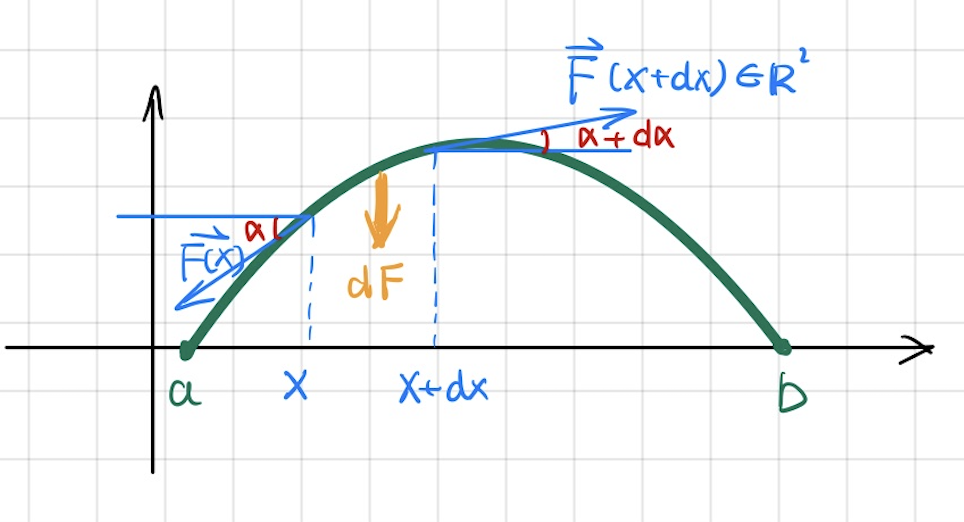
\includegraphics[width=0.6\textwidth]{graph.png}
\caption{弹性图。}
\end{figure}

\( F(x + dx) - F(x) = P \)

垂直分量是
\[
|F(x)| \sin(\alpha) = P \cos(\alpha) \text{ 等。}
\]

结果力 \( dF \) 是
\[
P (\sin(\alpha + d\alpha) - \sin(\alpha)) \approx P (\tan(\alpha + d\alpha) - \tan(\alpha)) 
\]
\[
= P (u'(x + dx) - u'(x))
\]

通过泰勒展开得到 \( P (u'(x) + u''(x)dx + O(dx^2) - u'(x)) \)

因此 \( dF = P u''(x) dx \) 作用在单位上

现在 \( u(x,t) = u(x) \)

牛顿第二定律 \( u''(x) = \frac{dF}{P dx} = \frac{P u''(x) dx}{P dx} \)

\subsection*{一维波动方程}

一维波动方程的初边值问题(IBVP):

\[
\begin{cases}
S u_{tt} = P u_{xx} + f(t,x), & \text{对于 } x \in (a,b),t > 0 \\
u(t,a) = u(t,b) = 0, & \text{对于 } t > 0 \\
u(0,x) = u_0(x), & \text{对于 } x \in (a,b) \\
u_{t}(0,x) = v_0(x), & \text{对于 } x \in (a,b)
\end{cases}
\]

其中 \( S \) 和 \( P \) 是常数,\( f(t,x) \) 是给定函数。

BC 表示迪里希特边界条件,附在这里。

IC 代表系统位置和速度的初始条件。

\subsection*{变形弦的势能}
\[
dE_{pot} = P \left( \sqrt{1 + u_{x}^2} - 1 \right) dx \approx P \left( \frac{1}{2} u_{x}^2 \right) dx
\]

使用泰勒展开,我们得到:
\[
dE_{pot} = \frac{P}{2} u_{x}^2 dx
\]

\subsection*{弦的能量平衡}

弦的总能量 \( E \) 是潜在能量和动能的总和:
\[
E = E_{pst} + E_{kin} = \int_{a}^{b} \frac{P}{2} u_{x}^2 dx + \int_{a}^{b} \frac{S}{2} u_{t}^2 dx
\]

关于时间的能量变化为:
\[
\frac{dE}{dt} = \int_{a}^{b} P u_{x} u_{xt} dx + \int_{a}^{b} S u_{t} u_{tt} dx
\]

使用链式法则和部分积分,我们得到:
\[
\int_{a}^{b} u_{x} u_{xt} dx = u u_{t} \Big|_{a}^{b} - \int_{a}^{b} u u_{xtt} dx = -\int_{a}^{b} u u_{xtt} dx
\]
因为由于迪里希特边界条件,\( u(t,a) = u(t,b) = 0 \)。

\subsection*{备注}

如果 \( t \neq 0 \),则关于时间的能量变化为:
\[
\frac{dE}{dt} = \int_{a}^{b} S u_{t} u_{tt} dx
\]

在稳态状态下,其中 \( u_{tt} = 0 \),我们有 \( P u_{xx} = 0 \) 在 \( (a,b) \) 内。



\subsection*{关于二维波动方程的备注}

考虑一个代表无阻力弯曲的二维材料的薄膜。所施加的力是 \( f(t,x) \)。

\[
S u_{tt} = P (\Delta u_{xx} + \Delta u_{yy}) + f
\]

或者更紧凑的形式为,

\[
S u_{tt} = P \Delta u + f
\]

其中 \( S \) 和 \( P \) 是与薄膜属性有关的常数,\( \Delta \) 是表示空间维度中二阶偏导数之和的拉普拉斯算子,\( f \) 是表示施加在薄膜上的外部力的函数。

\begin{figure}[h!]
\centering
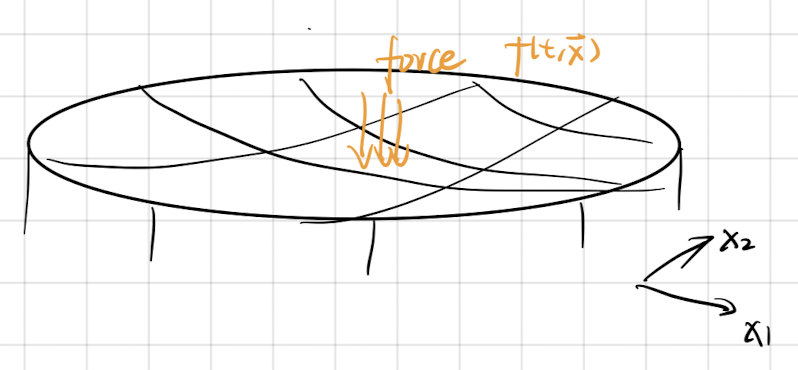
\includegraphics[width=0.5\textwidth]{membrane.png}
\caption{二维波动方程在薄膜上的示意图。}
\end{figure}

\newpage
\date{21.11.2023.PDE}
\section*{纵波(弹性理论的一维理论)}

参考构型:

- 拉伸和压缩粒子表示法。

从拉格朗日坐标(初始)到欧拉坐标的映射:
\[
\mathbf{X} \mapsto \mathbf{x} = \mathbf{X} + \mathbf{u}(t,\mathbf{x})
\]
其中 \( \mathbf{u}(t,\mathbf{x}) \) 是位移。

应变(局部变形):
\[
\epsilon(\mathbf{x}) = u'(\mathbf{x}) = \frac{d\mathbf{u}}{d\mathbf{x}} - 1
\]
\[
\begin{cases} 
\epsilon > 0 & \text{拉伸} \\
\epsilon < 0 & \text{压缩}
\end{cases}
\]

应力:
\[
\sigma(\mathbf{X}) = a(\mathbf{X}) \epsilon(\mathbf{X})
\]
其中 \( a(\mathbf{X}) \) 是材料参数(刚度)。

导致的力(应力的局部变化):
\[
\tilde{\mathbf{f}}(\mathbf{x}) = \sigma'(\mathbf{x})
\]
其中 \( \tilde{\mathbf{f}}(\mathbf{x}) \) 是力密度。

在受力 \( \sigma(\mathbf{x}) \) 和 \( \sigma(\mathbf{x} + d\mathbf{x}) \) 作用下的长度微元 \( d\mathbf{x} \) 上的结果力 \( \Delta \mathbf{F} \)。
% 您可以根据需要继续使用方程和表示。

% 微分力
微分力由以下公式给出:
\[
d\mathbf{F} = \sigma (\mathbf{x} + d\mathbf{x}) - \sigma (\mathbf{x}) = \sigma'(\mathbf{x})d\mathbf{x}, \quad \frac{d\mathbf{F}}{d\mathbf{x}} = \tilde{\mathbf{f}}
\]

% 偏微分方程(PDE)
纵波的PDE为:
\[
\mathbf{u}_{tt} = (a(\mathbf{x})\mathbf{u})' + \tilde{\mathbf{f}}(t,\mathbf{x})
\]
其中 \( \mathbf{u}_{tt} \) 是位移的二阶时间导数,\( \tilde{\mathbf{f}} \) 代表外部力。

% 边界条件(BC)
\begin{enumerate}
    \item 边界条件(例如,对于 \( t > 0 \),\( u(t,a) = u(t,b) = 0 \))
    \item 初始条件(例如,\( u(0,x) \) 和 \( u_t(0,x) \))
\end{enumerate}

% 2维薄膜的更一般形式
对于2维薄膜,PDE为:
\[
\mathbf{u}_{tt} = \nabla \cdot (a(\mathbf{x})\nabla \mathbf{u}) + \mathbf{f}(t,\mathbf{x}) \text{ 在 } \Omega \text{ 中,对于 } t > 0
\]

% 2维薄膜的边界条件
\begin{enumerate}
    \item 迪里希特边界条件(BC):\( u = 0 \) 在 \( \Gamma_1 \) 上,对于 \( t > 0 \)
    \item 诺依曼边界条件(BC):\( \mathbf{n}^T (a(\mathbf{x})\nabla u) = p \) 在 \( \Gamma_2 \) 上,对于 \( t > 0 \)(\( \Gamma_2 \) 上的力密度)
\end{enumerate}

% 2维薄膜的初始条件
初始条件(IC):\( u(0,\mathbf{x}) = u_0(\mathbf{x}) \) 和 \( u_t(0,\mathbf{x}) = v_0(\mathbf{x}) \) 在 \( \Omega \) 上

% 对于稳态PDE和能量平衡的备注
备注:稳态PDE类似于热方程的稳态状态。

% 能量平衡
能量平衡方程:
\begin{align*}
E &= \frac{1}{2} \int_{\Omega} \epsilon u \cdot (a(\mathbf{x})\nabla u) \, d\Omega + \frac{1}{2} \int_{\Omega} u_t^2 \, d\Omega \\
\frac{dE}{dt} &= \frac{1}{2} \int_{\Omega} 2 u_t (\nabla \cdot (a(\mathbf{x})\nabla u)) \, d\Omega + \int_{\Omega} u_{tt} u_t \, d\Omega - \int_{\Omega} \mathbf{f} \cdot \math

\subsection*{进一步的方程}

\begin{enumerate}
    \item 依赖于 \( u \) 的通量 \( \mathbf{J} \) 的输运方程:(一阶)
    % 在这里添加具体的输运方程
    
    \item 板的弯曲(2阶)/ 抵抗弯曲:比较梁的弯曲(1维)
    \begin{align*}
        \mathbf{u}_{itt} &= - \alpha \Delta u, \quad \text{其中} \quad \alpha = \frac{Eh^3}{12(1-\nu^2)} \\
        \text{对于梁} \quad \mathbf{u}_{itt} &= - \beta (\mathcal{R}u)''(x'')
    \end{align*}
    
    \item 静止电场。
    \begin{align*}
        \mathbf{E} &= \mathbf{E}_0(\mathbf{x}) \quad \text{(电场)} \\
        \mathbf{D} &= \mathbf{D}(\mathbf{x}) \quad \text{(电位移)} \\
        \rho &= \epsilon_0 \mathbf{E} \quad \text{(介电常数)} \\
        \mathbf{D}(\mathbf{x}) &= \epsilon(\mathbf{x}) \mathbf{E}(\mathbf{x}) \\
        \rho &= \rho(\mathbf{x}) \quad \text{(电荷密度)} \\
        \nabla \cdot \mathbf{D}(\mathbf{x}) &= \rho(\mathbf{x}) \\
        \Phi &= \Phi(\mathbf{x}) \quad \text{(电势)} \\
        -\nabla \Phi(\mathbf{x}) &= \mathbf{E}(\mathbf{x}) \\
        -\nabla \cdot (\epsilon(\mathbf{x}) \nabla \Phi(\mathbf{x})) &= \rho(\mathbf{x})
    \end{align*}
    与静态变形进行比较。
    \begin{align*}
        -\nabla \cdot (a(\mathbf{x}) \nabla u(\mathbf{x})) &= f(\mathbf{x})
    \end{align*}
    
    \item 流体流动的Navier-Stokes方程 \( \mathbf{u} = \mathbf{u}(\mathbf{x},t) \):
    \begin{align*}
        \frac{\partial \mathbf{u}}{\partial t} + (\mathbf{u} \cdot \nabla) \mathbf{u} &= \nu \Delta \mathbf{u} - \nabla p, \quad \text{其中 } p \text{ 是压力,} \nu \text{ 是粘度} \\
        \text{对于质量加速度:} \quad \frac{d \mathbf{u}}{d t} &= \frac{\partial \mathbf{u}}{\partial t} + \mathbf{u} \cdot \nabla \mathbf{u} \quad \text{(物质导数)}
    \end{align*}
\end{enumerate}

\newpage
\date{28.11.2023 PDE}

\section*{弹性变形:无限小变形的弹性理论,线性理论}

\begin{enumerate}
    \item 变形构型:
    \begin{itemize}
        \item 变形映射 \( \mathbf{\Lambda} \colon \mathcal{U} \to \mathbb{R}^3 \)
        \item 带有位移的映射 \( \mathbf{\Lambda} \colon \mathbf{X} \to \mathbf{x} = \mathbf{X} + \mathbf{u}(\mathbf{X}) \)
        \item 参考构型 \( \mathcal{U} \subset \mathbb{R}^3 \)
    \end{itemize}
    
    \item 刚体变换:
    \begin{itemize}
        \item 旋转矩阵 \( \mathbf{W} \),\( \mathbf{W}^T \mathbf{W} = \mathbf{I} \)
        \item 平移向量 \( \mathbf{t} \),使得 \( \mathbf{x} = \mathbf{W} \mathbf{X} + \mathbf{t} \)
    \end{itemize}
    
    \item 变形梯度 \( \nabla \mathbf{X} \):
    \begin{itemize}
        \item \( \mathbf{F} = \mathbf{I} + \nabla \mathbf{u} \)
        \item Cauchy-Green应变张量 \( \mathbf{E} = \frac{1}{2} (\nabla \mathbf{X}^T \nabla \mathbf{X} - \mathbf{I}) \)
        \item 对于小变形:\( \mathbf{E} \approx \mathbf{I} + \nabla \mathbf{u} + (\nabla \mathbf{u})^T \)
    </itemize>

    \item 线性化的Cauchy-Green应变:
    \begin{itemize}
        \item \( \mathbf{E} = \frac{1}{2} (\nabla \mathbf{u}^T + \nabla \mathbf{u}) \)
        \item 应变的近似 \( \mathbf{e} \approx \mathbf{I} + 2\mathbf{E} \)
        \item 刚体平移 \( \mathbf{x} = \mathbf{X} + \mathbf{t} \),\( \nabla \mathbf{t} = \mathbf{0} \in \mathbb{R}^{3\times3} \),\( \boldsymbol{\epsilon} = \mathbf{0} \in \mathbb{R}^{3\times3} \)
        \item 旋转矩阵 \( \mathbf{W} \) 和应变张量 \( \boldsymbol{\epsilon} \) 用于旋转角度 \( \phi \) 的旋转:
        \[
        \mathbf{W} =
        \begin{pmatrix}
            \cos \phi & -\sin \phi & 0 \\
            \sin \phi & \cos \phi & 0 \\
            0 & 0 & 1
        \end{pmatrix}
        , \quad
        \boldsymbol{\epsilon} =
        \begin{pmatrix}
            \cos \phi - 1 & \sin \phi & 0 \\
            -\sin \phi & \cos \phi - 1 & 0 \\
            0 & 0 & 0
        \end{pmatrix}
        \]
        \item 注意:对于小角度旋转,几何刚度,即仅适用于小角度旋转的线性理论。
    \end{itemize}
\end{enumerate}
\textit{线性材料法则:胡克定律。}


\section*{应力和运动方程}

应力张量 \( \mathbf{\sigma}(\mathbf{X}) \) 与刚度张量 \( \mathbf{S}(\mathbf{X}) \) 和应变张量 \( \boldsymbol{\epsilon}(\mathbf{X}) \) 的关系:
\[
\mathbf{\sigma}(\mathbf{X}) = \mathbf{S}(\mathbf{X}) \colon \boldsymbol{\epsilon}(\mathbf{X})
\]
其中 \( \mathbf{S} \) 有36个分量,但由于对称性(6个独立分量),只有21个唯一分量。

应力张量的矩阵表示形式:
\[
\mathbf{\sigma} =
\begin{pmatrix}
\sigma_{11} & \sigma_{12} & \sigma_{13} \\
\sigma_{21} & \sigma_{22} & \sigma_{23} \\
\sigma_{31} & \sigma_{32} & \sigma_{33}
\end{pmatrix}
\]

结果力 \( \mathbf{f} \) 由应力张量的散度给出:
\[
\mathbf{f} = \nabla \cdot \mathbf{\sigma}
\]

弹性连续体的运动方程:
\[
\mathbf{u}_{tt} = \nabla \cdot \mathbf{\sigma} + \mathbf{f} \quad \text{对于} \quad \mathbf{X} \in \Omega, t > 0
\]

边界条件 (BC):
\[
\mathbf{u} = \mathbf{g} \quad \text{对于} \quad \mathbf{X} \in \Gamma_1, t > 0
\]
\[
\mathbf{n} \cdot \mathbf{\sigma} = \mathbf{p} \quad \text{对于} \quad \mathbf{X} \in \Gamma_2, t > 0
\]

初始条件 (IC):
\[
\mathbf{u}(0,\mathbf{X}) = \mathbf{u}_0(\mathbf{X}) \quad \text{和} \quad \mathbf{u}_t(0,\mathbf{X}) = \mathbf{v}_0
\]

各向同性线性材料模型和用 Lamé 常数 \( \lambda \) 和 \( \mu \) 表示的胡克定律:
\[
\mathbf{\sigma} = \lambda \text{tr}(\boldsymbol{\epsilon}) \mathbf{I} + 2\mu \boldsymbol{\epsilon}
\]
\[
\text{其中 tr}(\boldsymbol{\epsilon}) = \epsilon_{11} + \epsilon_{22} + \epsilon_{33} \quad \text{(应变张量的迹,即体积变化)}
\]

Lamé 常数与杨氏模量 \( E \) 和泊松比 \( \nu \) 相关:
\[
\lambda = \frac{\nu E}{(1+\nu)(1-2\nu)} \quad \text{和} \quad \mu = \frac{E}{2(1+\nu)}
\]

Lamé 算子 \( \mathbf{L} \) 与应力张量梯度相关:
\[
\mathbf{L} \mathbf{u} = \nabla \cdot \mathbf{\sigma}
\]

应力-应变关系的散度形式:
\[
\nabla \cdot \mathbf{\sigma} = (\lambda + \mu) \nabla (\nabla \cdot \mathbf{u}) + \mu \Delta \mathbf{u}
\]

当体力 \( \mathbf{f} \) 为零时的特殊情况:
\[
\mathbf{\sigma} \cdot \mathbf{n} = \mathbf{0}, \quad \nabla \cdot \mathbf{\sigma} = \mathbf{0}
\]
对于 \( \mathbf{f} = \mathbf{0} \)。


\section*{PDE 的分类}

\subsection*{线性 PDE}
线性偏微分方程(PDE)涉及线性微分算子。PDE 的阶数是涉及的导数的阶数。

\begin{itemize}
    \item 一阶 PDE 通常更容易处理。
    \item 二阶 PDE 更复杂。
\end{itemize}

\subsection*{二阶线性 PDE}
对于定义在域 \( \Omega \subset \mathbb{R}^d \) 上的二阶线性 PDE,矩阵 \( A \) 是对称的,其中单位矩阵表示为 \( I \)。

\subsubsection*{1. 扩散或热方程}
原型扩散方程,也称为热方程,表现出均匀化行为:
\[
u_{t} - \nabla \cdot (A \nabla u) = f
\]
这的原型是 \( u_{t} = \Delta u \),可以离散为:
\[
u_{it} - \Delta u = u_{it} - u_{i+1,j} - u_{i,j+1} - \cdots - u_{i+1,j+1} + f
\]

\subsubsection*{2. 波动方程}
用于弹性变形导致的波动传播和振荡:
\[
\mathbf{u}_{tt} - \nabla \cdot (A \nabla \mathbf{u}) = \mathbf{f}
\]
这的原型波动方程是 \( u_{tt} = \Delta u \)。

\subsubsection*{3. 静态问题}
示例包括弹性薄膜或热扩散的静态问题:
\[
-\nabla \cdot (A \nabla u) = f
\]

\subsubsection*{椭圆型 PDE}
椭圆型 PDE 的原型是泊松方程:
\[
-\Delta u = f
\]

\subsection*{最大值原理}
对于没有外力的附加薄膜,最大值原理表明解 \( u \) 在边界 \( \partial\Omega \) 上取得最大值:
\[
-\Delta u = 0 \quad \text{在} \quad \Omega, \quad u = g \quad \text{在} \quad \partial\Omega
\]
函数 \( u \) 在 \( \partial\Omega \) 上取得最大值。


最后三张插图展示了不同类型偏微分方程(PDEs)适用的边界条件(BCs)。

1. **对于抛物型方程**,通常模拟像热传导这样的时间依赖过程。初始条件(ICs)在时间 \( t = 0 \) 时给出,边界条件(BCs)沿着空间域 \( \Omega \) 的边界 \( \partial\Omega \) 给出。这种方程关注一个区域随时间的变化,通常需要在起始时间定义初始状态,以及在空间边界上定义边界条件。

2. **对于双曲型方程**,常用于模拟波的传播。初始条件(ICs)在时间 \( t = 0 \) 时给出,边界条件(BCs)同样沿着空间域 \( \Omega \) 的边界 \( \partial\Omega \) 给出。双曲型方程与波动和振动有关,需要知道初始的波形和边界上的波动行为。

3. **对于椭圆型方程**,通常与静态状态相关,如静电势问题。边界条件(BCs)沿着整个空间域 \( \Omega \) 的边界 \( \partial\Omega \) 给出。椭圆型方程描述了平衡状态,通常只需要在边界上设置条件。

每种方程类型的边界和初始条件选择是为了确保数学模型正确描述物理现象,并能够找到方程的解。

\begin{figure}[h]
\centering
\begin{minipage}[b]{0.3\linewidth}
\centering
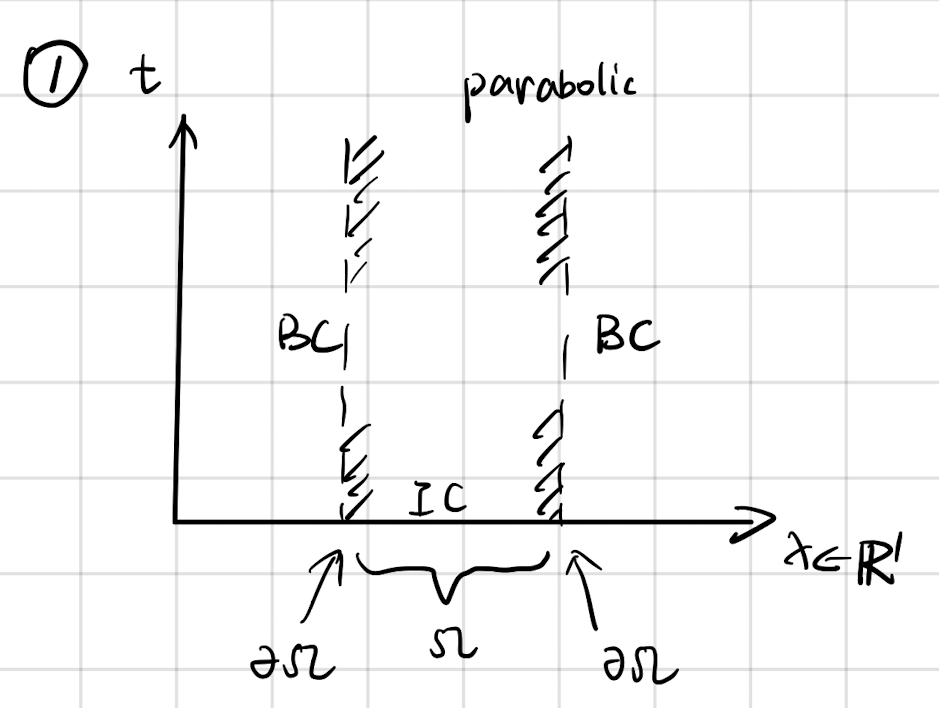
\includegraphics[width=\textwidth]{path_to_parabolic_BC_diagram}
\caption{Parabolic BCs and ICs}
\end{minipage}
\hspace{0.5cm}
\begin{minipage}[b]{0.3\linewidth}
\centering
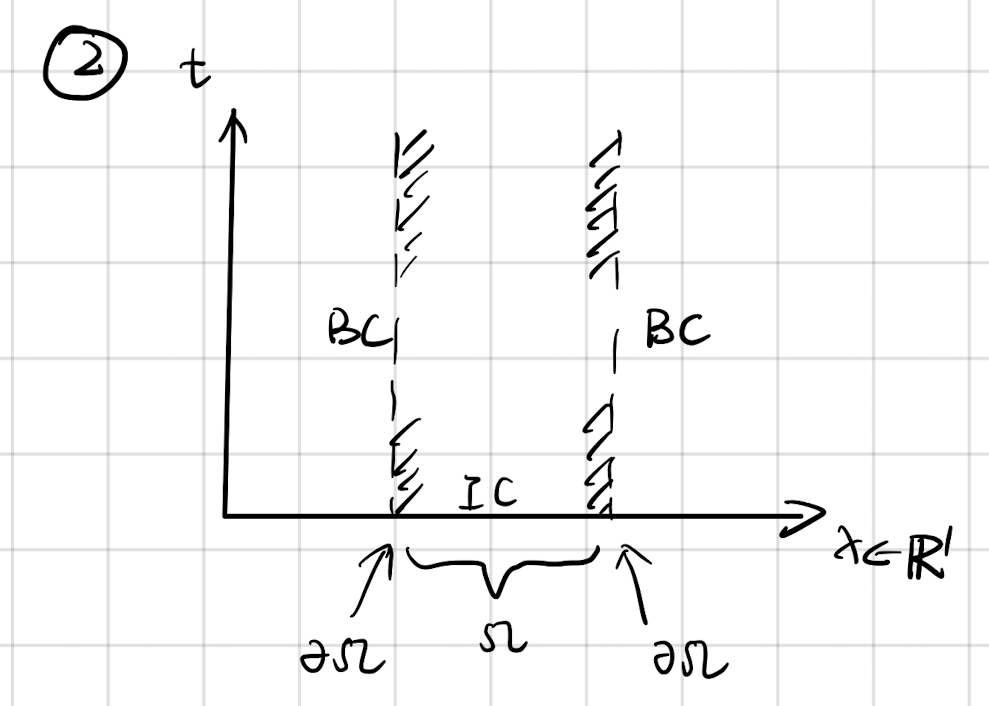
\includegraphics[width=\textwidth]{path_to_hyperbolic_BC_diagram}
\caption{Hyperbolic BCs and ICs}
\end{minipage}
\hspace{0.5cm}
\begin{minipage}[b]{0.3\linewidth}
\centering
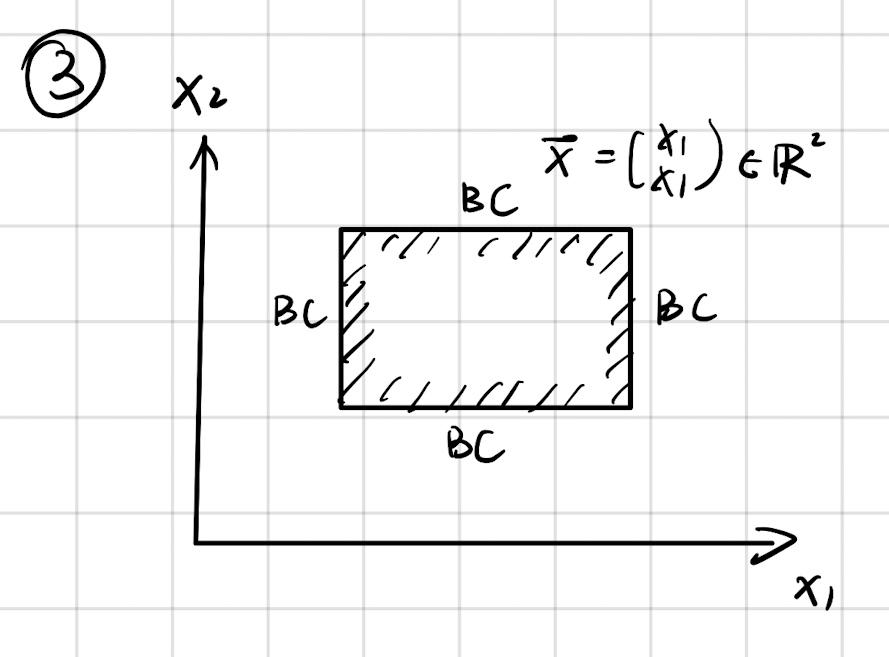
\includegraphics[width=\textwidth]{path_to_elliptic_BC_diagram}
\caption{Elliptic BCs}
\end{minipage}
\end{figure}





\section*{III. Simple Solution Techniques}

\subsection*{III.1. Parabolic Differential Equation in Homogeneous Form}

Homogeneous Dirichlet Boundary Conditions (BCs) on domain $\Omega = (0, L)$:

\begin{align*}
\text{PDE} \quad & u_t = a u_{xx} & \text{for } x \in (0,L), t > 0 \\
\text{BC} \quad & u(t,0) = u(t,L) = 0 & \text{for } t \geq 0 \\
\text{IC} \quad & u(0,x) = u_0(x) & \text{for } x \in (0,L) \\
\end{align*}

Product approach / ansatz $u(t,x) = U(t)V(x)$:

PDE $\rightarrow U(t)V(x) = aU(t)V''(x)$

Separation of the variables:

\[
\frac{U'(t)}{U(t)} = a\frac{V''(x)}{V(x)} = -\lambda^2 \text{ (constant)}.
\]

Independent of $x$ implies constant.

$\rightarrow$ ODE $aV''(x) \sim V(x)$

BC $U(t)V(0) = U(t)V(L) = 0$

$U(t) = 0$ provides $u \equiv 0$, boring.

$\Rightarrow V(0) = V(L) = 0$

\[
V(x) = \sin \frac{k\pi x}{L} \text{ with } k = 1,2,3,\ldots
\]

\[
aV''(x) = -a \left(\frac{k\pi}{L}\right)^2 V(x) \Rightarrow U'(t) = -a \left(\frac{k\pi}{L}\right)^2 U(t)
\]

\[
\Rightarrow U(t) = Ce^{-a\left(\frac{k\pi}{L}\right)^2 t}, \quad C \in \mathbb{R}
\]

For every $k = 1,2,3,\ldots$ we get the solutions:

\[
u(t,x) = Ce^{-a\left(\frac{k\pi}{L}\right)^2 t} \sin \frac{k\pi x}{L}, \quad C \in \mathbb{R}
\]

Coefficient $\beta_k$

PDE (linear $\rightarrow$ linear combination are solution):

\[
u(t,x) = \sum_{k=1}^{\infty} \beta_k e^{-a\left(\frac{k\pi}{L}\right)^2 t} \sin \frac{k\pi x}{L}
\]

\subsection*{Example: $L = \pi, a = 1, u = \sum \beta_k e^{-k^2 t} \sin kx$}

IC:

\[
u(0,x) = \sum_{k=1}^{\infty} \beta_k \sin \frac{k\pi x}{L} = u_0(x) \quad \text{(x)}
\]

Orthogonal with respect to $L^2([0,L])$.

Represents $f,g \in L^2([0,L])$:

\[
\langle f, g \rangle_{L^2([0,L])} = \int_0^L f(x) g(x) dx
\]



Now multiply $(x)$ by $\sin \frac{l\pi x}{L}, \ l = 1,2,3,\ldots$:

\begin{align*}
\int_0^L \sum_{k=1}^{\infty} \beta_k \sin \frac{k\pi x}{L} \sin \frac{l\pi x}{L} dx &= \int_0^L u_0(x) \sin \frac{l\pi x}{L} dx \\
\sum_{k=1}^{\infty} \beta_k \int_0^L \sin \frac{k\pi x}{L} \sin \frac{l\pi x}{L} dx &= \frac{L}{2} \delta_{kl} = \begin{cases} 0 & \text{for } k \neq l \\ \frac{L}{2} & \text{for } k = l \end{cases}
\end{align*}

Hence,

\begin{align*}
\frac{L}{2} \beta_l &= \int_0^L u_0(x) \sin \frac{l\pi x}{L} dx \\
\text{or} \quad \beta_l &= \frac{2}{L} \int_0^L u_0(x) \sin \frac{l\pi x}{L} dx
\end{align*}

Fourier coefficients can be computed for all $u_0 \in L^2([0, L])$.




\subsection*{Inhomogeneous Boundary Conditions (BCs).}

\begin{align*}
\text{PDE} \quad & u_{t} = a u_{xx}, & x \in (0, L), t > 0 \\
\text{BC} \quad & u(t,0) = q_1, \ u(t,L) = q_2 \in \mathbb{R}, & \text{for } t \geq 0 \\
\text{IC} \quad & u(0,x) = u_0(x), & x \in (0,L) \\
\end{align*}

\[
w(x) = q_1 + \frac{q_2 - q_1}{L} x
\]

$v + w = u$ with $v_{t} = u_{t}$ and $v_{xx} = u_{xx}$

Boundary Value Problem (BVP) for $v$
\begin{align*}
\text{PDE} \quad & v_{t} = a v_{xx}, & x \in (0, L), t > 0 \\
\text{BC} \quad & v(t,0) = v(t,L) = 0, & t > 0 \\
\text{IC} \quad & v(0,x) = u_0(x) - w(x), & x \in (0,L) \\
\end{align*}

\section*{II. Spectral Decomposition}

\begin{align*}
\text{PDE} \quad & u_{t} = a u_{xx} + f(t,x), & x \in (0, L), t > 0 \\
\text{BC} \quad & u(t,0) = u(t,L) = 0, & t > 0 \\
\text{IC} \quad & u(0,x) = u_0(x), & \\
\end{align*}

Approach $u(t,x) = \sum_{k=1}^{\infty} V_k(t) \sin\left(\frac{k \pi x}{L}\right)$

\begin{itemize}
\item $V_k(t)$ -- time-dependent intensity.
\item $\sin\left(\frac{k \pi x}{L}\right)$ -- eigenmodes.
\end{itemize}

\begin{align*}
u_{t} &= \sum_{k=1}^{\infty} V_k'(t) \sin\left(\frac{k \pi x}{L}\right) \\
u_{xx} &= \sum_{k=1}^{\infty} V_k(t) \left(-\frac{k \pi}{L}\right)^2 \sin\left(\frac{k \pi x}{L}\right) \\
f(t,x) &= \sum_{k=1}^{\infty} F_k(t) \sin\left(\frac{k \pi x}{L}\right) \\
u_0(x) &= \sum_{k=1}^{\infty} M_k \sin\left(\frac{k \pi x}{L}\right) \\
\end{align*}

\begin{itemize}
\item $\sin\left(\frac{k \pi x}{L}\right)$ eigenmodes are pairwise orthogonal so they are linear independent.
\end{itemize}




\section*{II.2. Spectral Decomposition}

Consider the PDE with spectral decomposition:
\begin{align*}
\text{PDE} \quad & u_{t} = a u_{xx} + f(t,x), & x \in (0,L), t > 0 \\
\text{BC} \quad & u(t,0) = u(t,L) = 0, & t \geq 0 \\
\text{IC} \quad & u(0,x) = u_0(x), & \\
\end{align*}

The approach for the solution:
\[ u(t,x) = \sum_{k=1}^{\infty} V_k(t) \sin\left(\frac{k\pi x}{L}\right) \]
where \( V_k(t) \) represents the time-dependent intensity and \( \sin\left(\frac{k\pi x}{L}\right) \) are the eigenmodes.

The temporal and spatial derivatives are given by:
\begin{align*}
u_t &= \sum_{k=1}^{\infty} V_k'(t) \sin\left(\frac{k\pi x}{L}\right), \\
u_{xx} &= \sum_{k=1}^{\infty} V_k(t) \left(-\left(\frac{k\pi}{L}\right)^2\right) \sin\left(\frac{k\pi x}{L}\right).
\end{align*}

Let the inhomogeneity \( f(t,x) \) and the initial condition \( u_0(x) \) be represented as:
\begin{align*}
f(t,x) &= \sum_{k=1}^{\infty} f_k(t) \sin\left(\frac{k\pi x}{L}\right), \\
u_0(x) &= \sum_{k=1}^{\infty} M_k \sin\left(\frac{k\pi x}{L}\right),
\end{align*}
where the eigenmodes \( \sin\left(\frac{k\pi x}{L}\right) \) are pairwise orthogonal and linearly independent.

Upon equating coefficients, we get an ordinary differential equation for each mode \( V_k(t) \):
\[ V_k'(t) = -a\left(\frac{k\pi}{L}\right)^2 V_k(t) + f_k(t), \]
with the initial condition \( V_k(0) = M_k \).

The spectral decomposition for the PDE for each single mode \( \delta_k = \delta_k(t) \) is:
\[ u_k(t) = -a\left(\frac{k\pi}{L}\right)^2 V_k(t) + \alpha_k(t), \]
where \( \alpha_k(t) \) represents the coefficients of the inhomogeneity in the mode \( k \).

\textbf{Remark:} Higher frequency modes, i.e., higher \( k \) values, fade out faster due to the factor \( -a\left(\frac{k\pi}{L}\right)^2 \) in the spectral decomposition.


Example: string on $\Omega = (0,\pi)$ with inner and outer damping.

\begin{align*}
\delta u_{tt} + d_{out} u_{t} &= P u_{xx} + d_{in} u_{xxt}, & x \in (0,\pi), t > 0 \\
\delta \sum_{k=1}^{\infty} \delta_k''(t) \sin(kx) &+ (d_{out} + k^2 d_{in}) \delta_k'(t) + P k^2 \delta_k(t) = 0
\end{align*}

Every intensity $\delta_k$ follows the ODE of a one-way oscillator.


\end{document}



\end{document}

\end{document}


\maketitle